\section{Methodology}

\subsection{Multimodal Input Representation}
To avoid ambiguity between symbolic variables and sensor names, we represent each observation using an ordered multimodal feature vector:
\begin{equation}
\mathbf{x} = [x, y, \text{TEMP}, \text{COR}_{A}, \text{COR}_{V}] \in \mathbb{R}^{5},
\end{equation}
and a three-output target vector:
\begin{equation}
\mathbf{y} = [\text{pH}, \text{OD}, \text{TURB}] \in \mathbb{R}^{3}.
\end{equation}
Input features are normalized before spike encoding. We then apply rate coding so that each normalized scalar is converted into a spike train over $T$ time steps, with firing probability proportional to its magnitude. This produces a temporal representation compatible with the downstream LIF dynamics while preserving the multimodal structure of the original sample.

\subsection{SNN Architecture}
The model follows a feed-forward SNN with topology $5 \rightarrow 64 \rightarrow 3$, with a hidden leaky integrate-and-fire (LIF) layer, as illustrated in Fig.~\ref{fig:proposed_arch}. The membrane update is
\begin{equation}
\mathbf{u}_{t+1} = \beta\,\mathbf{u}_{t} + \mathbf{W}\mathbf{s}_{t} - \theta\,\mathbf{z}_{t},
\end{equation}
where $\beta$ is membrane decay, $\theta$ is firing threshold, and $\mathbf{z}_t$ are emitted spikes. Output prediction is computed by temporal aggregation across steps.

\begin{figure}[!htbp]
\centering
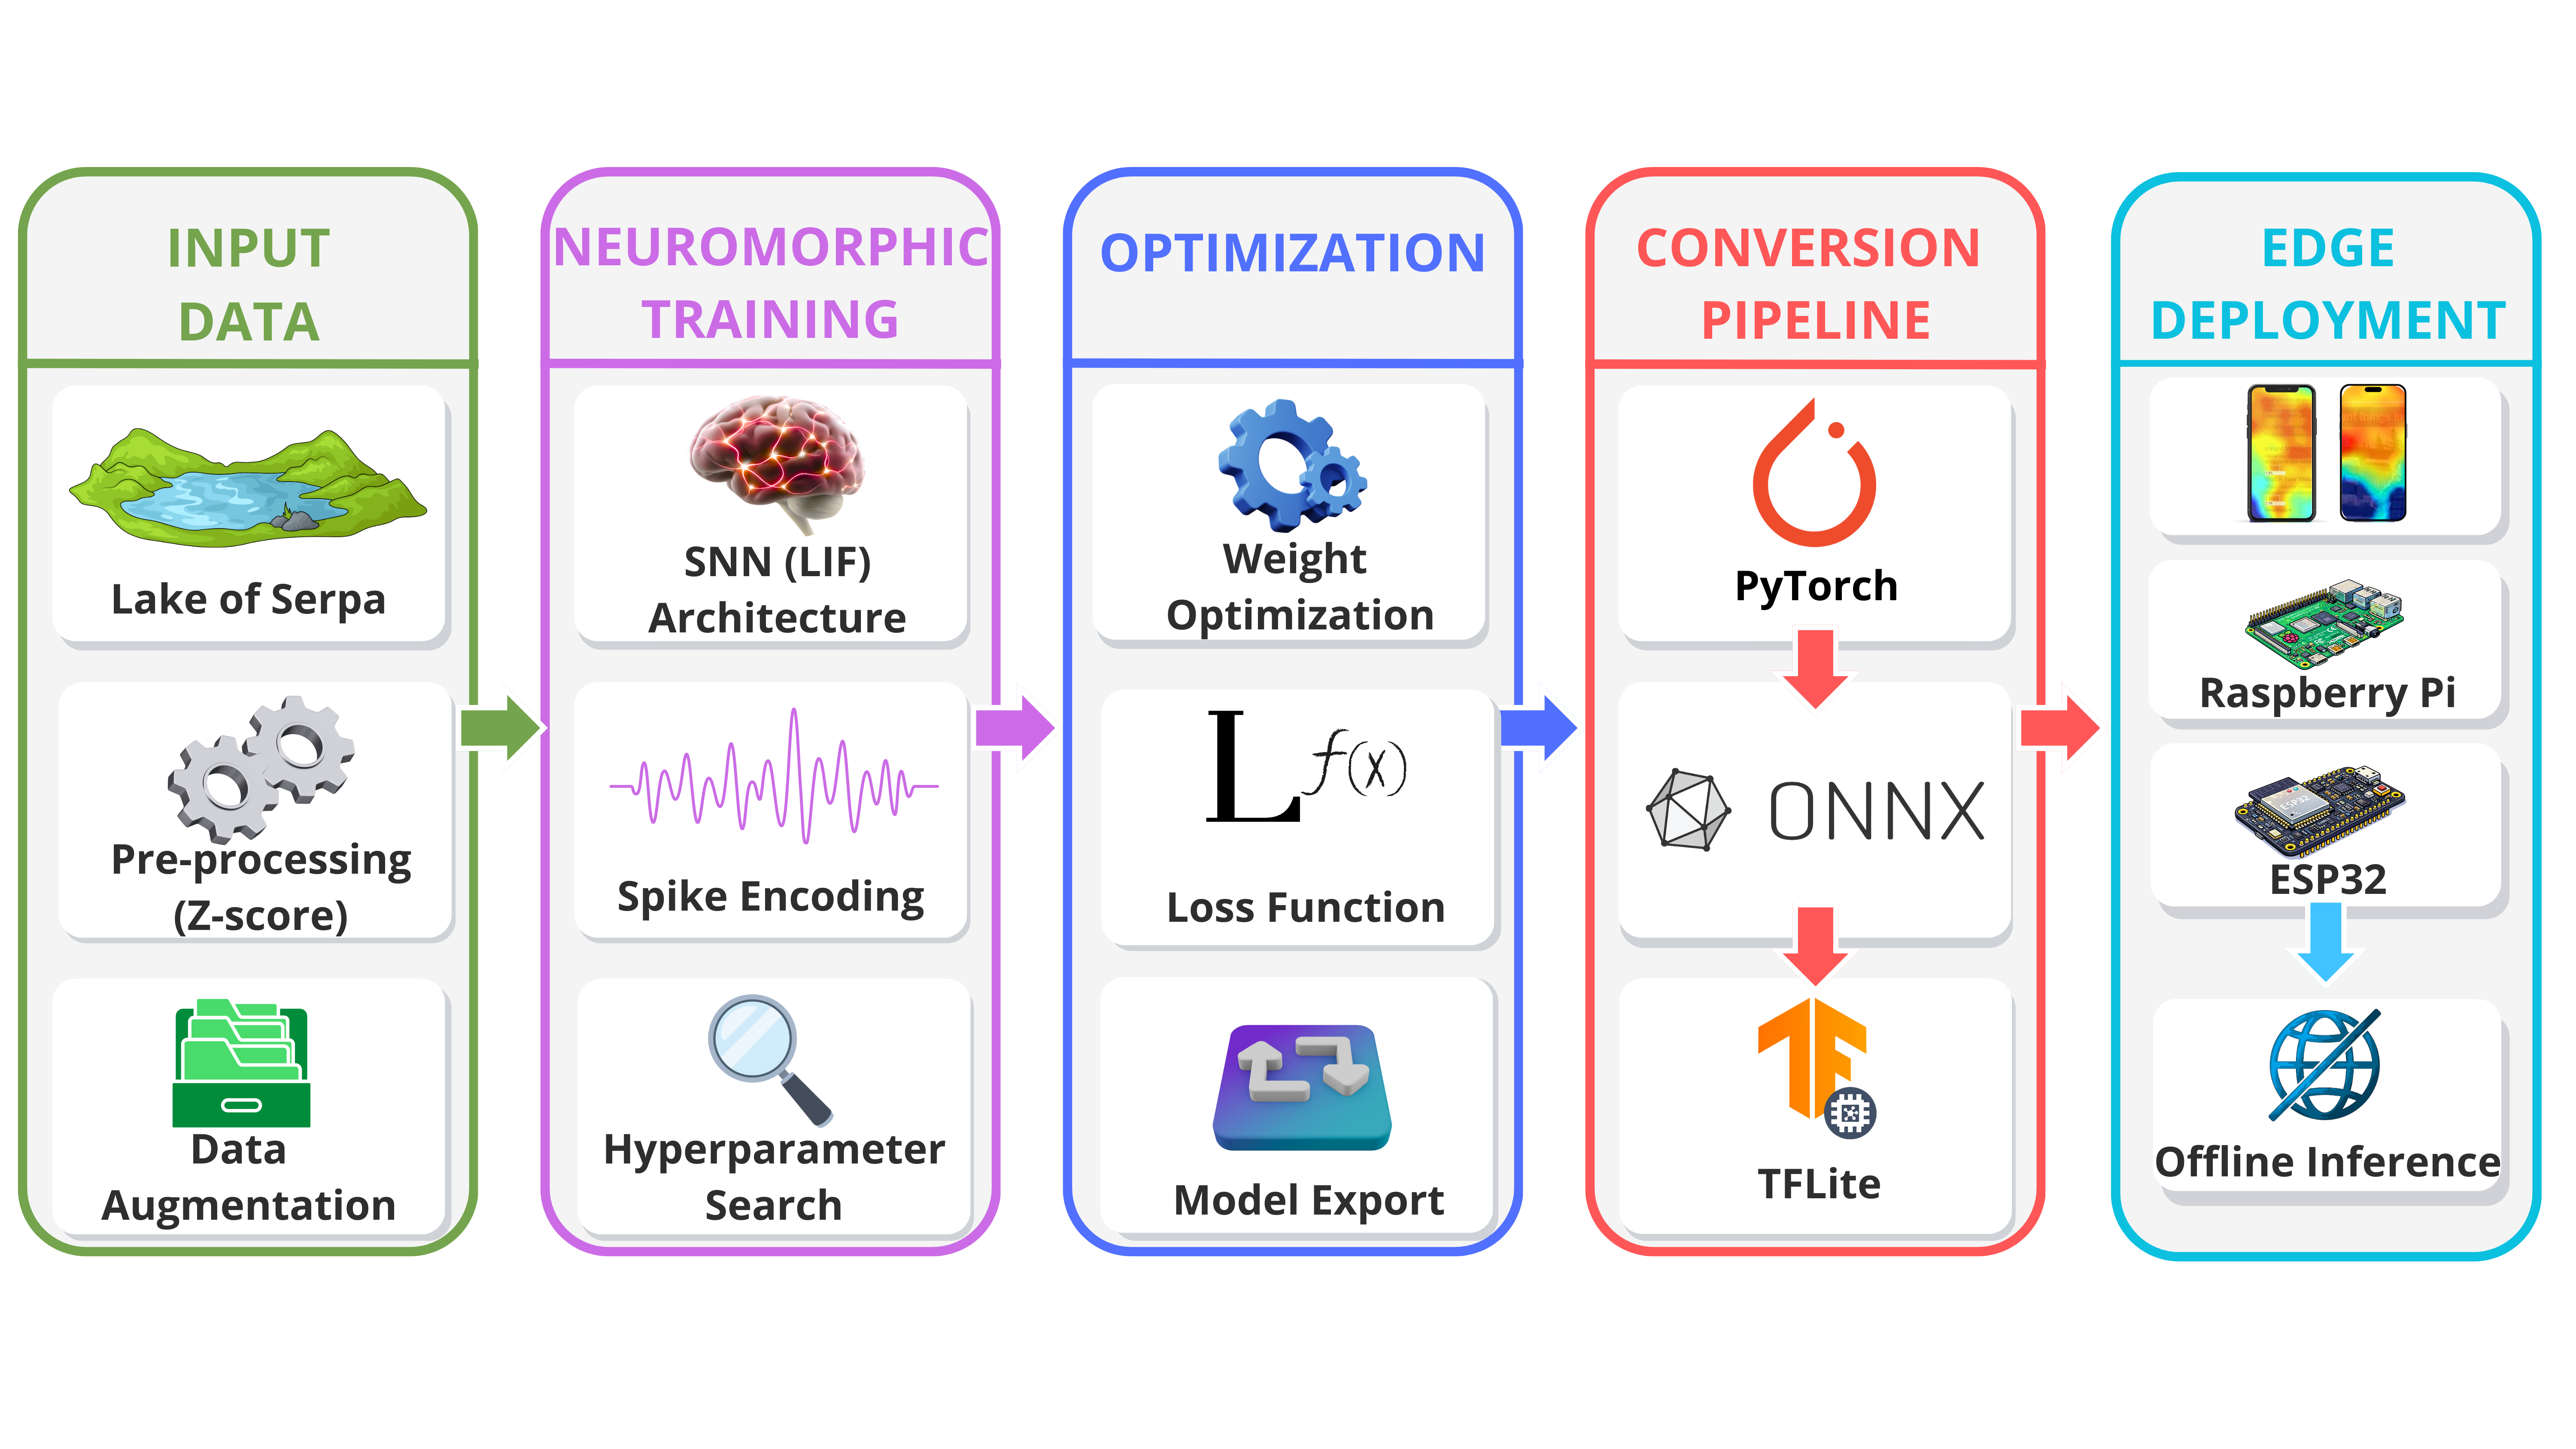
\includegraphics[width=0.86\textwidth]{Arquitetura.png}
\caption{Proposed multimodal SNN architecture for offline edge inference.}
\label{fig:proposed_arch}
\end{figure}

Figure~\ref{fig:proposed_arch} presents the complete end-to-end workflow adopted in this study. The first block consolidates field data preparation, including normalization and controlled augmentation. The second block represents neuromorphic training with LIF neurons, spike encoding, and hyperparameter search. The third block covers model optimization and export of trained parameters. The fourth block defines the interoperability path from PyTorch to ONNX and then to TFLite for lightweight runtime execution. Finally, the fifth block shows edge deployment on heterogeneous platforms (Android, Raspberry Pi, and ESP32), all operating under an offline inference paradigm suitable for low-connectivity monitoring scenarios.

\subsection{Training Protocol}
Training used Adam optimizer and weighted MSE loss with early stopping. Hyperparameters were selected by grid search over hidden size, learning rate, temporal steps $T$, threshold, and decay factor. Evaluation used repeated random seeds and macro metrics (MAE, RMSE, and $R^2$) over the three targets.

As shown in Fig.~\ref{fig:loss_curve_method}, both training and validation losses decrease rapidly in the initial epochs and then converge to a stable plateau with limited divergence. This behavior indicates that the selected configuration reached consistent optimization without strong overfitting patterns, supporting the use of early stopping and confirming that the augmented multimodal training setup improved convergence stability for this small-data regime.

\begin{figure}[!htbp]
\centering
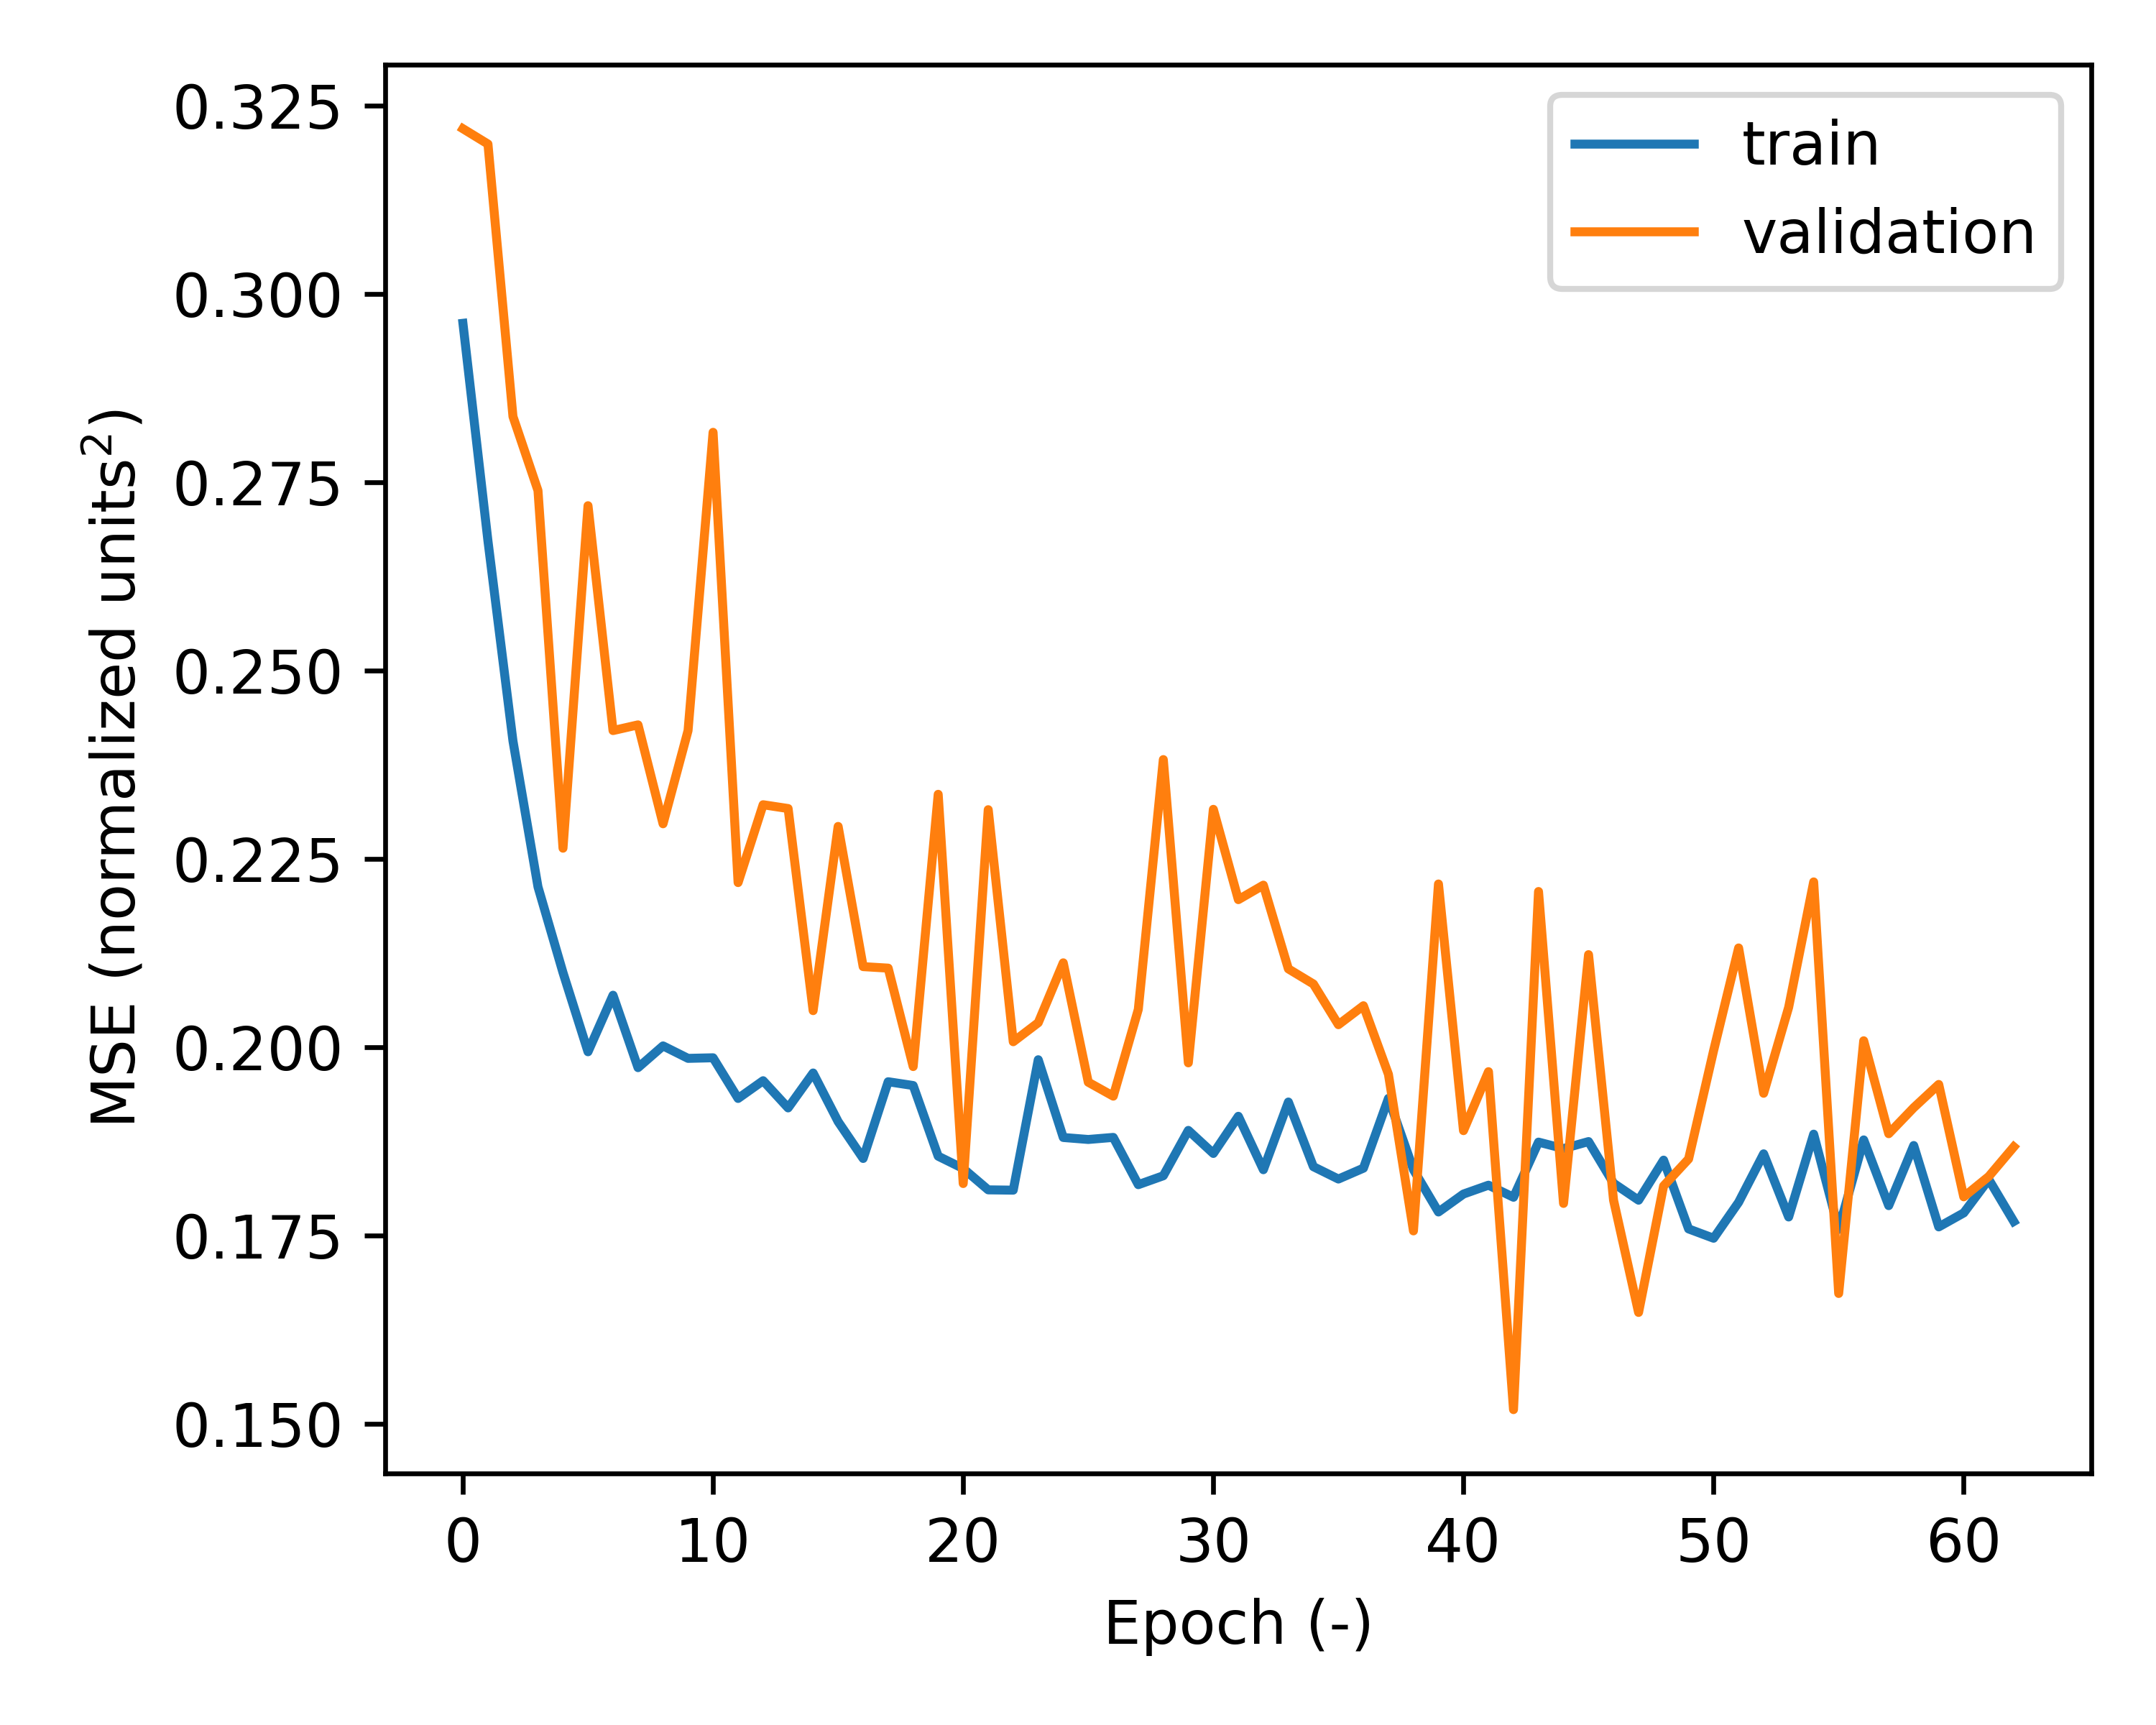
\includegraphics[width=0.5\textwidth]{loss_curve_multi.png}
\caption{Training and validation loss (MSE) of the selected multimodal SNN.}
\label{fig:loss_curve_method}
\end{figure}



\FloatBarrier
